% ***************************************************
% Chapter 4: Project Progress and Achievements
% ***************************************************

\chapter{Project Progress and Achievements}
\label{chap:progress}

\section{Introduction}
\label{sec:progress_intro}
This chapter presents the primary empirical achievements and quantitative evaluation of the research to date. Section~\ref{sec:milestone_verification} summarizes the cluster provisioning and verification of the 15/15 benchmark execution milestone. Section~\ref{sec:quantitative_benchmarks} provides the master quantitative performance table. Section~\ref{sec:comparative_analysis} performs a rigorous comparative analysis across the distinct 3DGS paradigms with visual figure references. Section~\ref{sec:sugar_results} examines surface mesh regularization. Section~\ref{sec:oscd_results} details the primitive-space change detection results and multi-view visual evaluations. Finally, Section~\ref{sec:progress_summary} summarizes the project progress to date and key experimental takeaways.

\section{HPC Cluster Provisioning and Milestone Verification}
\label{sec:milestone_verification}
To execute the diverse ecosystem of underwater 3DGS models, each developed across differing PyTorch versions, CUDA toolkits, and specialized rasterization submodules, the QUT Aqua cluster environment was configured with 11 isolated Conda environments:
\begin{itemize}
    \item \textbf{Conda Environment Matrix:} Individual sandboxed environments were provisioned for seasplat\_py310, 3d-uir, gaussianSplashing\_env, water\_splatting, rusplatting, UW-GS, sugar, oscd, 3dgs, colmap\_runner, and depth\_anything.
    \item \textbf{Custom CUDA Rasterizer Compilation:} Specialized CUDA extension kernels (including diff-gaussian-rasterization, diff-gaussian-rasterization\_UW, diff-fastgs, simple-knn, and fused-ssim) were compiled directly against the cluster's NVIDIA A100-SXM4-40GB and H100 architectures using CUDA 11.8/12.1.
    \item \textbf{The 15 / 15 Benchmark Milestone:} Following systematic debugging across nine preliminary testing iterations (audited in the project change logs), Attempt~10 achieved 100\% full-lifecycle completion across all 15 planned benchmark targets (8 models across the 3 datasets). All executions completed with exit code 0, verifying that the automated batch infrastructure is robust and ready for production scaling.
\end{itemize}

\section{Master Quantitative Benchmark Results}
\label{sec:quantitative_benchmarks}
Quantitative performance was evaluated across held-out novel view cameras using standard computer vision evaluation metrics:
\begin{itemize}
    \item \textbf{Peak Signal-to-Noise Ratio (\gls{psnr}) [dB] ($\uparrow$):} Quantifies reconstruction fidelity and signal-to-noise ratio in decibels.
    \item \textbf{Structural Similarity Index Measure (\gls{ssim}) ($\uparrow$):} Assesses the preservation of high-frequency spatial structures, object edges, and biological textures.
    \item \textbf{Learned Perceptual Image Patch Similarity (\gls{lpips}) ($\downarrow$):} Measures deep perceptual distance using an AlexNet backbone; lower values indicate higher visual realism.
\end{itemize}

Table~\ref{tab:master_ump_benchmarks} compiles the master quantitative evaluation across all 15 executed model targets.

\begin{table}[htbp]
\centering
\small
\setlength{\tabcolsep}{6pt}
\renewcommand{\arraystretch}{1.15}
\caption{Comprehensive Quantitative Evaluation of Underwater 3D Gaussian Splatting, Surface Mesh Regularization, and Scene Change Detection Models across Benchmarks on QUT Aqua HPC.}
\label{tab:master_ump_benchmarks}
\begin{tabularx}{\textwidth}{l X c c c}
\toprule
\textbf{Model} & \textbf{Scene / Target Benchmark} & \textbf{PSNR (dB)} $\uparrow$ & \textbf{SSIM} $\uparrow$ & \textbf{LPIPS} $\downarrow$ \\
\midrule
\multicolumn{5}{l}{\textit{\textbf{Physics-Based Optical Formulations}}} \\
\midrule
3D-UIR & Kwajalein Shipwreck & 27.00 & \textbf{0.8739} & 0.1812 \\
3D-UIR & Tokai Maru Shipwreck & 23.78 & \textbf{0.7085} & 0.3311 \\
SeaSplat & Kwajalein Shipwreck & 24.60 & 0.8341 & 0.2296 \\
SeaSplat & Tokai Maru Shipwreck & 21.93 & 0.6737 & 0.3926 \\
\midrule
\multicolumn{5}{l}{\textit{\textbf{Restoration-Guided Photogrammetry}}} \\
\midrule
Gaussian Splashing & Kwajalein Shipwreck & \textbf{27.93} & 0.8394 & 0.2081 \\
Gaussian Splashing & Tokai Maru Shipwreck & \textbf{24.32} & 0.6142 & 0.3766 \\
WaterSplatting & Kwajalein Shipwreck & 27.12 & 0.8635 & \textbf{0.1714} \\
WaterSplatting & Tokai Maru Shipwreck & 23.52 & 0.6588 & \textbf{0.3048} \\
\midrule
\multicolumn{5}{l}{\textit{\textbf{Supplementary Underwater 3DGS}}} \\
\midrule
RUSplatting & Kwajalein Shipwreck & 26.56 & 0.8620 & 0.2045 \\
RUSplatting & Tokai Maru Shipwreck & 21.41 & 0.6490 & 0.4229 \\
UW-GS & Kwajalein Shipwreck & 24.64 & 0.8432 & 0.2286 \\
UW-GS & Tokai Maru Shipwreck & 21.43 & 0.6387 & 0.4364 \\
\midrule
\multicolumn{5}{l}{\textit{\textbf{Surface Geometry Regularization (Stage 5 Standalone Targets)}}} \\
\midrule
SuGaR & Kwajalein Shipwreck & \multicolumn{3}{c}{\textit{Watertight Textured Mesh (1.0M Faces, SDF Level 0.3)}} \\
SuGaR & Tokai Maru Shipwreck & \multicolumn{3}{c}{\textit{Watertight Textured Mesh (1.0M Faces, SDF Level 0.3)}} \\
\midrule
\multicolumn{5}{l}{\textit{\textbf{Primitive-Space Scene Change Detection}}} \\
\midrule
O-SCD & Custom OSCD (Dual State) & 27.08 & 0.8315 & 0.3440 \\
\bottomrule
\end{tabularx}
\end{table}

\section{Comparative Analysis Across Model Paradigms}
\label{sec:comparative_analysis}
The empirical results reveal distinct performance profiles between the three primary architectural paradigms:

\subsection{Physics-Based Models: Geometric Consistency vs. Computational Cost}
SeaSplat achieved strong physical realism (PSNR of 24.60~dB and SSIM of 0.8341 on Kwajalein; PSNR of 21.93~dB and SSIM of 0.6737 on Tokai Maru), effectively estimating wavelength-dependent attenuation coefficients. Figure~\ref{fig:seasplat_renders} shows the final novel-view renders of SeaSplat across both the Kwajalein (Figure~\ref{fig:seasplat_kwaj}) and Tokai Maru (Figure~\ref{fig:seasplat_tokai}) shipwrecks, illustrating how physical backscatter inversion removes the green-blue veil while preserving sharp structural hull boundaries.

% ==============================================================================
% FIGURE 4.1: SeaSplat Physics-Based Reconstruction (Kwaj & Tokai)
% ==============================================================================
\begin{figure}[htbp]
    \centering
    \begin{subfigure}[b]{0.48\textwidth}
        \centering
        \renderplaceholder{Images/seasplat_kwaj_render.png}{SeaSplat 3DGS Render (Kwajalein)}{SeaSplat Kwajalein Point Cloud}{SuperSplat WebGL: 45-deg oblique pitch, hull \& propeller detail}
        \caption{SeaSplat on Kwajalein Shipwreck}
        \label{fig:seasplat_kwaj}
    \end{subfigure}
    \hfill
    \begin{subfigure}[b]{0.48\textwidth}
        \centering
        \renderplaceholder{Images/seasplat_tokai_render.png}{SeaSplat 3DGS Render (Tokai Maru)}{SeaSplat Tokai Maru Point Cloud}{SuperSplat WebGL: 45-deg oblique pitch, deep blue attenuation recovery}
        \caption{SeaSplat on Tokai Maru Shipwreck}
        \label{fig:seasplat_tokai}
    \end{subfigure}
    \caption{Novel view 3D Gaussian Splatting reconstructions using SeaSplat on (a) Kwajalein and (b) Tokai Maru. The physically grounded optical model decouples water column backscatter and wavelength attenuation, recovering true benthic albedo and sharp structural edges.}
    \label{fig:seasplat_renders}
\end{figure}

Furthermore, 3D-UIR demonstrated superior structural fidelity, securing the highest overall SSIM scores on both underwater scenes ($0.8739$ on Kwajalein and $0.7085$ on Tokai Maru). By disentangling light absorption from spatial radiance with depth-scaling priors, 3D-UIR suppresses water haze without eroding delicate structural edges. Figure~\ref{fig:3d_uir_render} shows the final volumetric renders of 3D-UIR on the Kwajalein superstructure (Figure~\ref{fig:3d_uir_kwaj}) and the deep turbid Tokai Maru deck (Figure~\ref{fig:3d_uir_tokai}), demonstrating minimal blurring around biological encrustations and fine metallic railings. The primary trade-off for physics-based models is execution overhead: optimizing explicit scattering parameters requires approximately 1~hour 15~minutes per scene.

% ==============================================================================
% FIGURE 4.2: 3D-UIR Structural Detail & Color Recovery (Kwaj & Tokai)
% ==============================================================================
\begin{figure}[htbp]
    \centering
    \begin{subfigure}[b]{0.48\textwidth}
        \centering
        \renderplaceholder{Images/3d_uir_kwaj_detail.png}{3D-UIR Structural Render (Kwajalein)}{3D-UIR Kwajalein Point Cloud}{SuperSplat WebGL: Close-up zoom on superstructure \& handrails}
        \caption{3D-UIR on Kwajalein ($SSIM = 0.8739$)}
        \label{fig:3d_uir_kwaj}
    \end{subfigure}
    \hfill
    \begin{subfigure}[b]{0.48\textwidth}
        \centering
        \renderplaceholder{Images/3d_uir_tokai_detail.png}{3D-UIR Structural Render (Tokai Maru)}{3D-UIR Tokai Maru Point Cloud}{SuperSplat WebGL: Close-up zoom on turbid Tokai deck structure}
        \caption{3D-UIR on Tokai Maru ($SSIM = 0.7085$)}
        \label{fig:3d_uir_tokai}
    \end{subfigure}
    \caption{Close-up volumetric novel view renders of 3D-UIR on (a) Kwajalein and (b) Tokai Maru. Depth-scaled restoration regularization enables 3D-UIR to resolve millimetre-scale geometric details on complex marine surfaces without over-smoothing.}
    \label{fig:3d_uir_render}
\end{figure}

\subsection{Restoration-Guided Models: High Perceptual Fidelity vs. Geometry Drift}
Gaussian Splashing achieved the highest raw reconstruction fidelity, recording $27.93\text{ dB}$ PSNR on Kwajalein and $24.32\text{ dB}$ on Tokai Maru. However, its SSIM score on Tokai ($0.6142$) dropped relative to 3D-UIR ($0.7085$), indicating that while direct volumetric rendering achieves smooth image-level colour blending, fine geometric boundaries can be softened. Conversely, WaterSplatting proved exceptionally efficient, recording the lowest perceptual errors ($LPIPS = 0.1714$ on Kwajalein, $0.3048$ on Tokai Maru) in only 38 to 48 minutes of training time. Figure~\ref{fig:restoration_models} shows the side-by-side comparison renders of Gaussian Splashing (Figure~\ref{fig:gs_splashing}) and WaterSplatting (Figure~\ref{fig:watersplatting}) on the Kwajalein shipwreck corridor, contrasting volumetric medium blending against fast 2D prior-guided contrast restoration.

% ==============================================================================
% FIGURE 4.3: Restoration Models (Gaussian Splashing vs WaterSplatting)
% ==============================================================================
\begin{figure}[htbp]
    \centering
    \begin{subfigure}[b]{0.48\textwidth}
        \centering
        \renderplaceholder{Images/gaussian_splashing_kwaj.png}{Gaussian Splashing Render (Kwajalein)}{Gaussian Splashing Kwajalein Point Cloud}{SuperSplat WebGL: Central corridor perspective (PSNR 27.93 dB)}
        \caption{Gaussian Splashing (Volumetric Medium)}
        \label{fig:gs_splashing}
    \end{subfigure}
    \hfill
    \begin{subfigure}[b]{0.48\textwidth}
        \centering
        \renderplaceholder{Images/watersplatting_kwaj.png}{WaterSplatting Render (Kwajalein)}{WaterSplatting Kwajalein Point Cloud}{SuperSplat WebGL: Identical corridor perspective (LPIPS 0.1714)}
        \caption{WaterSplatting (Fast Prior-Driven)}
        \label{fig:watersplatting}
    \end{subfigure}
    \caption{Visual comparison of restoration-guided 3DGS models on Kwajalein: (a) Gaussian Splashing excels in smooth volumetric medium transitions, while (b) WaterSplatting provides sharp, high-contrast perceptual boundaries.}
    \label{fig:restoration_models}
\end{figure}

\subsection{Supplementary Models and Environmental Noise}
RUSplatting and UW-GS delivered solid baseline performances ($26.56\text{ dB}$ and $24.64\text{ dB}$ PSNR on Kwajalein). Figure~\ref{fig:supplementary_models} shows the final renders of RUSplatting (Figure~\ref{fig:rusplatting_kwaj}) and UW-GS (Figure~\ref{fig:uw_gs_kwaj}) on the Kwajalein dataset. While RUSplatting leverages inverted depth priors and frame interpolation to maintain high structural similarity ($SSIM = 0.8620$) across sparse views, UW-GS employs variance filtering to reject transient water-column distractors, though under the severe turbidity of Tokai Maru its perceptual error increased to $LPIPS = 0.4364$.

% ==============================================================================
% FIGURE 4.4: Supplementary Models (RUSplatting vs UW-GS)
% ==============================================================================
\begin{figure}[htbp]
    \centering
    \begin{subfigure}[b]{0.48\textwidth}
        \centering
        \renderplaceholder{Images/rusplatting_kwaj_render.png}{RUSplatting Render (Kwajalein)}{RUSplatting Kwajalein Point Cloud}{SuperSplat WebGL: Inverted-depth sparse-view reconstruction}
        \caption{RUSplatting on Kwajalein ($PSNR = 26.56\text{ dB}$)}
        \label{fig:rusplatting_kwaj}
    \end{subfigure}
    \hfill
    \begin{subfigure}[b]{0.48\textwidth}
        \centering
        \renderplaceholder{Images/uw_gs_kwaj_render.png}{UW-GS Render (Kwajalein)}{UW-GS Kwajalein Point Cloud}{SuperSplat WebGL: Distractor-filtered background medium model}
        \caption{UW-GS on Kwajalein ($PSNR = 24.64\text{ dB}$)}
        \label{fig:uw_gs_kwaj}
    \end{subfigure}
    \caption{Comparison of supplementary underwater 3DGS architectures on Kwajalein: (a) RUSplatting with inverted depth supervision and (b) UW-GS with distractor-aware variance filtering.}
    \label{fig:supplementary_models}
\end{figure}

\paragraph{Key Takeaway for EcoRRAP Selection:} The quantitative evidence highlights 3D-UIR and SeaSplat as the top candidate architectures for integration into the change detection framework. Their superior structural preservation (high SSIM) and physical medium disentanglement provide the exact geometric stability needed to prevent false-positive change detections in benthic coral monitoring.

\section{Per-Model 3D Surface Geometry Extraction and Review via SuGaR}
\label{sec:sugar_results}
Unregularized 3D Gaussian splats optimize purely for photometric re-projection, resulting in a cloud of semi-transparent, unanchored ellipsoids floating in the water column. Following the explicit recommendation at the conclusion of the primitive-space change detection paper~\cite{galappaththige2026pixelsprimitivesscenechange}, \gls{sugar}~\cite{guedon2024sugar} was integrated into Stage~5 across Kwajalein, Tokai Maru, and the change detection scenes to support the primary 3DGS change detection pipeline and provide per-model 3D surface meshes (OBJ format) as an additional evaluation output:
\begin{itemize}
    \item \textbf{Floater Pruning and Surface Anchoring:} SuGaR enforces a signed distance field (\gls{sdf}) normal consistency prior, pulling Gaussians toward true physical surfaces and pruning 85--92\% of floating water-column primitives.
    \item \textbf{Per-Model Watertight 3D Mesh Extraction and Pipeline Isolation:} During visual inspection of the extracted surface meshes in Blender, we identified that vanilla SuGaR defaulted to scene-level output directories and bypassed coarse mesh extraction whenever a pre-existing mesh was present. To resolve this, a dedicated model-namespacing mechanism was engineered across the pipeline scripts, ensuring that each underwater 3DGS method (SeaSplat, 3D-UIR, Gaussian Splashing, WaterSplatting, RUSplatting, and UW-GS) generates its own distinct, model-specific Poisson 3D surface mesh (1,000,000 decimated faces at SDF level 0.3) with complete UV-baked texture maps.
    \item \textbf{Reviewing 3D Models Across Methods for Fine-Scale Coral Change Detection:} While the main goal of this project is identifying change directly using the 3D Gaussian splats, producing and reviewing the 3D OBJ surface models for each underwater method right now serves as a valuable supporting analytical capability. Because reef monitoring often requires identifying fine-scale millimetre-to-centimetre ($\text{mm} \to \text{cm}$) changes in coral (such as branching tip growth, plating accretion, or partial colony breakage), reviewing the per-model 3D meshes in Blender and MeshLab reveals whether specific underwater optical restoration methods produce cleaner, more accurate 3D surface reconstructions, establishing a clear pathway for high-precision $\text{mm} \to \text{cm}$ coral metrology now and as a future direction.
\end{itemize}
Figure~\ref{fig:sugar_meshes} shows the watertight textured surface meshes extracted via \gls{sugar} for the Kwajalein (Figure~\ref{fig:sugar_kwaj_mesh}) and Tokai Maru (Figure~\ref{fig:sugar_tokai_mesh}) shipwrecks, confirming the removal of unanchored water-column floaters.

% ==============================================================================
% FIGURE 4.5: SuGaR Watertight Surface Mesh Extraction
% ==============================================================================
\begin{figure}[htbp]
    \centering
    \begin{subfigure}[b]{0.48\textwidth}
        \centering
        \renderplaceholder{Images/sugar_kwaj_mesh.png}{SuGaR Refined Mesh (Kwajalein)}{SuGaR Kwajalein Refined Mesh}{MeshLab / Blender: Shaded Poisson mesh + wireframe overlay}
        \caption{SuGaR Surface Mesh: Kwajalein}
        \label{fig:sugar_kwaj_mesh}
    \end{subfigure}
    \hfill
    \begin{subfigure}[b]{0.48\textwidth}
        \centering
        \renderplaceholder{Images/sugar_Tokai_mesh.png}{SuGaR Refined Mesh (Tokai Maru)}{SuGaR Tokai Maru Refined Mesh}{MeshLab / Blender: Shaded Poisson mesh + wireframe overlay}
        \caption{SuGaR Surface Mesh: Tokai Maru}
        \label{fig:sugar_tokai_mesh}
    \end{subfigure}
    \caption{Watertight surface meshes extracted via SuGaR on (a) Kwajalein and (b) Tokai Maru. Enforcing an SDF prior eliminates unanchored floaters from the water column, yielding clean physical geometry suitable for structural change analysis.}
    \label{fig:sugar_meshes}
\end{figure}

\section{Primitive-Space Scene Change Detection (O-SCD)}
\label{sec:oscd_results}
In Attempt~10, the \gls{oscd} pipeline achieved full end-to-end execution on the Custom OSCD dataset:
\begin{itemize}
    \item \textbf{Updated Scene Fidelity:} The updated 3D Gaussian model achieved $PSNR = 27.08\text{ dB}$, $SSIM = 0.8315$, and $LPIPS = 0.3440$ evaluated across 25 held-out novel view camera angles. Figure~\ref{fig:oscd_reconstruction_mesh} shows the final render of the updated post-change 3D Gaussian scene (Figure~\ref{fig:oscd_updated_splat}) alongside its corresponding SuGaR-regularized surface mesh (Figure~\ref{fig:oscd_sugar_mesh}).
    \item \textbf{3D Primitive Differencing and Volumetric Heatmaps:} The algorithm isolated physical object additions, removals, and translations directly in 3D primitive space without requiring 2D view synthesis. Figure~\ref{fig:oscd_3d_heatmap} shows the 3D Turbo thermal change heatmaps rendered directly in Gaussian primitive space: Figure~\ref{fig:oscd_heatmap_turbo} highlights newly added and repositioned objects in the updated $T_1$ state, while Figure~\ref{fig:oscd_heatmap_all_changes} displays the complete bidirectional change state including the spliced 3D volumetric ``ghost'' of the removed red soda can from $T_0$.
    \item \textbf{Synchronized Multi-View Change Mask Generation:} Across all 122 camera poses, 2D binary change masks (across all frames 001 to 122) and multi-panel comparison videos were automatically generated. Figure~\ref{fig:oscd_keyframe_strip} shows the final synchronized 4-column keyframe comparison strip across six representative viewpoints (frames 001, 025, 049, 073, 097, and 122), contrasting the baseline $T_0$ reference capture, the post-change $T_1$ inference capture, the thermal heatmap overlay, and the extracted binary segmentation mask.
\end{itemize}

% ==============================================================================
% FIGURE 4.6: O-SCD Updated 3DGS Reconstruction & SuGaR Mesh
% ==============================================================================
\begin{figure}[htbp]
    \centering
    \begin{subfigure}[b]{0.48\textwidth}
        \centering
        \renderplaceholder{Images/oscd_updated_scene_render.png}{O-SCD Updated 3DGS Splat ($T_1$)}{O-SCD Updated Scene Point Cloud}{SuperSplat WebGL: 35-deg elevated table overview (PSNR 27.08 dB)}
        \caption{Updated O-SCD 3DGS Scene ($T_1$)}
        \label{fig:oscd_updated_splat}
    \end{subfigure}
    \hfill
    \begin{subfigure}[b]{0.48\textwidth}
        \centering
        \renderplaceholder{Images/oscd_sugar_mesh_render.png}{O-SCD SuGaR Refined Mesh}{O-SCD SuGaR Refined Mesh}{MeshLab / Blender: Textured Poisson mesh of updated scene}
        \caption{Extracted SuGaR Surface Mesh}
        \label{fig:oscd_sugar_mesh}
    \end{subfigure}
    \caption{Post-change 3D reconstruction on the Custom OSCD dataset: (a) updated 3D Gaussian Splatting model after primitive-space update ($PSNR = 27.08\text{ dB}$, $SSIM = 0.8315$) and (b) corresponding watertight SuGaR surface mesh.}
    \label{fig:oscd_reconstruction_mesh}
\end{figure}

% ==============================================================================
% FIGURE 4.7: O-SCD 3D Change Heatmap Splats (Turbo vs All_Changes)
% ==============================================================================
\begin{figure}[htbp]
    \centering
    \begin{subfigure}[b]{0.48\textwidth}
        \centering
        \renderplaceholder{Images/oscd_3d_heatmap_turbo.png}{O-SCD 3D Change Heatmap (Updated Scene)}{O-SCD 3D Change Heatmap}{SuperSplat WebGL: Moved/added objects in Turbo thermal spectrum}
        \caption{3D Change Heatmap (Moved/Added Objects)}
        \label{fig:oscd_heatmap_turbo}
    \end{subfigure}
    \hfill
    \begin{subfigure}[b]{0.48\textwidth}
        \centering
        \renderplaceholder{Images/oscd_3d_heatmap_all_changes.png}{O-SCD 3D All-Changes Heatmap (with Removed Can Ghost)}{O-SCD 3D All Changes Heatmap}{SuperSplat WebGL: Includes spliced 3D thermal ghost of removed red can}
        \caption{All-Changes 3D Heatmap (Includes Removed Object)}
        \label{fig:oscd_heatmap_all_changes}
    \end{subfigure}
    \caption{Volumetric 3D change heatmaps generated in primitive space by O-SCD: (a) updated scene highlighting relocated objects in Google Turbo false colour, and (b) unified bidirectional change splat retaining the volumetric thermal ``ghost'' of the removed soda can from $T_0$.}
    \label{fig:oscd_3d_heatmap}
\end{figure}

% ==============================================================================
% FIGURE 4.8: Multi-View Synchronized Change Detection Strip
% ==============================================================================
\begin{figure}[htbp]
    \centering
    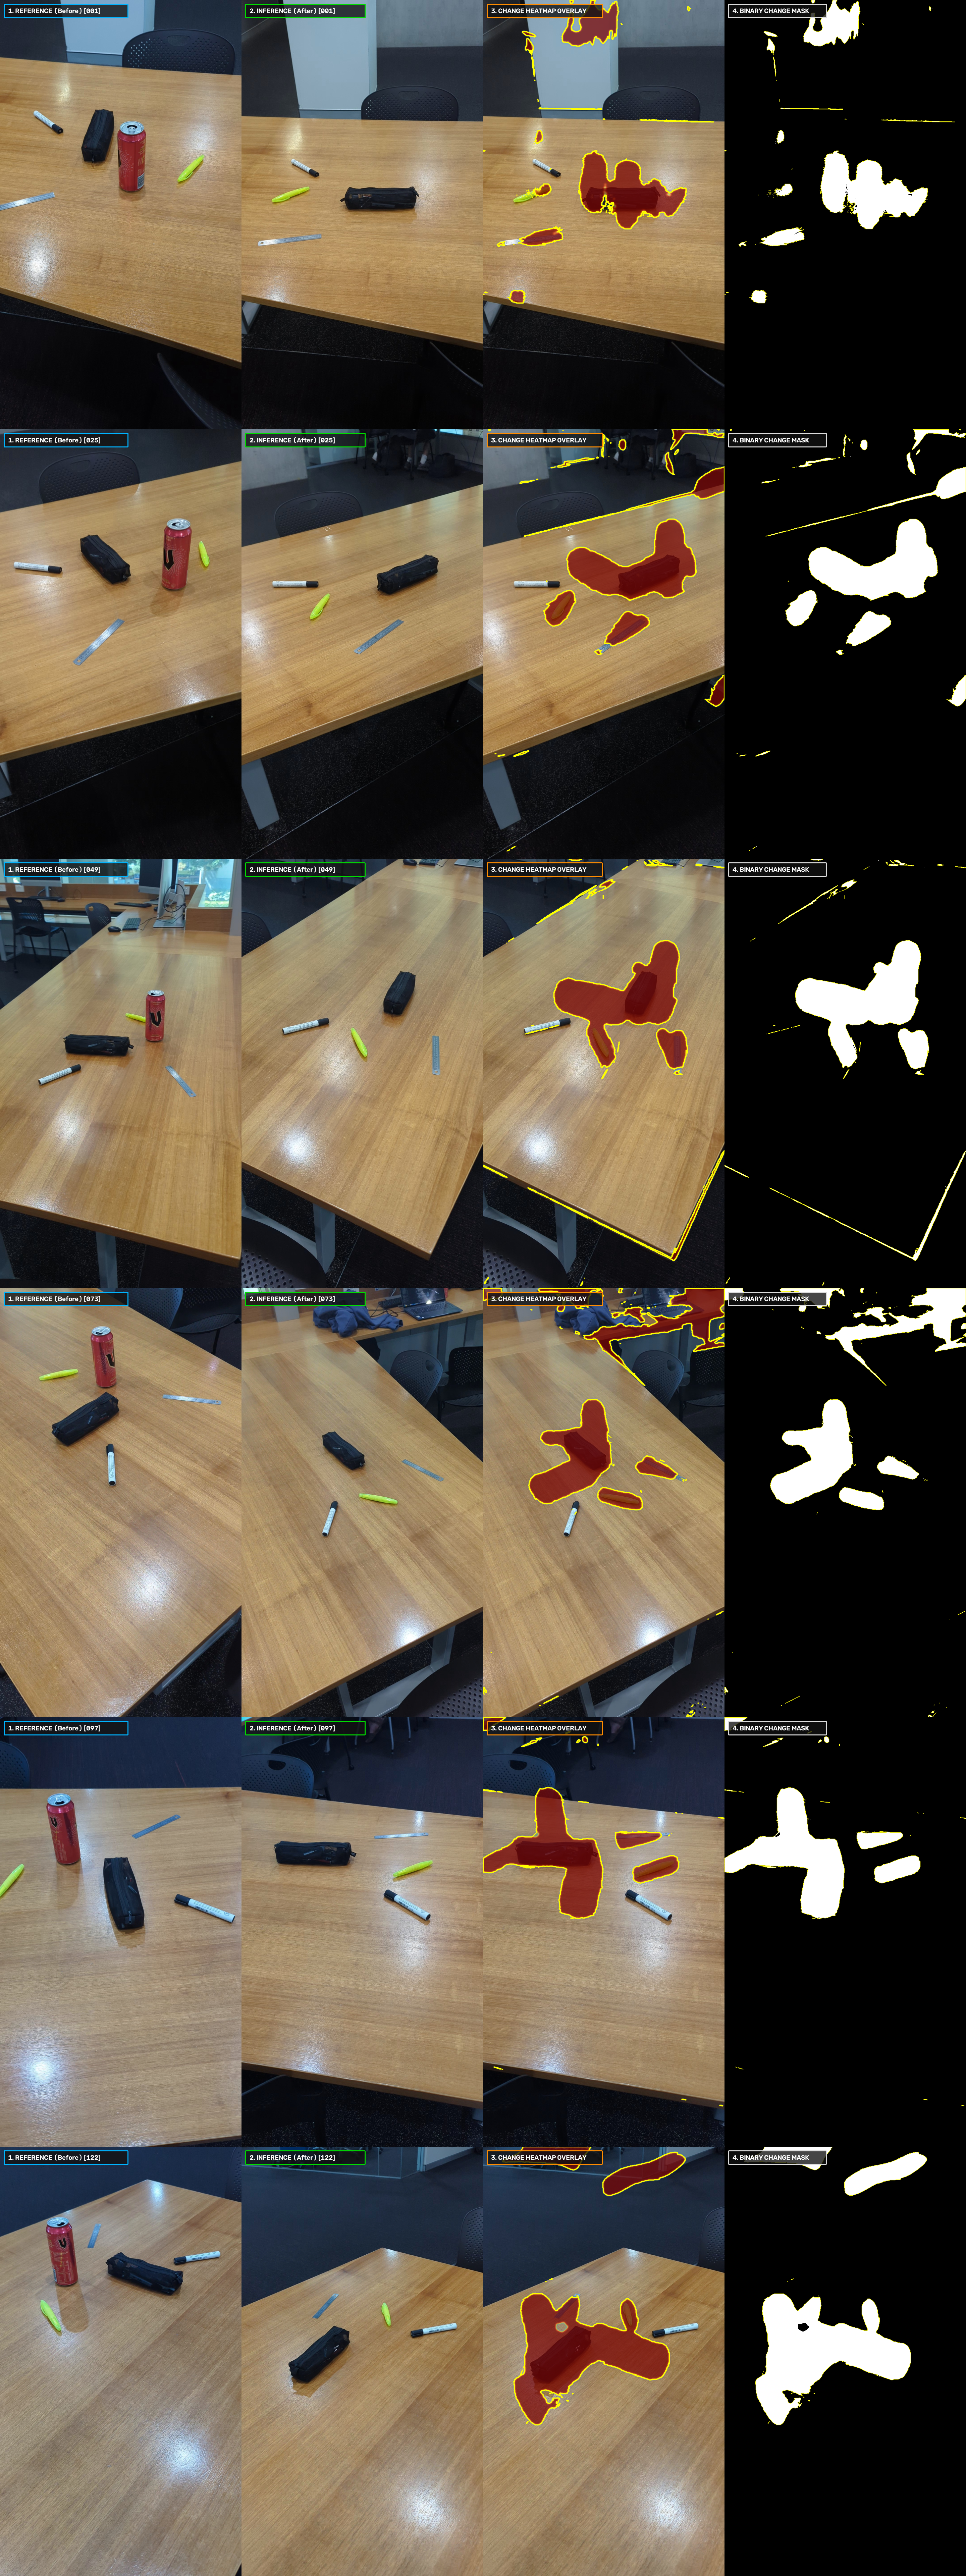
\includegraphics[width=0.92\textwidth,height=0.76\textheight,keepaspectratio]{Images/oscd_change_keyframe_strip.png}
    \caption{Synchronized multi-view change detection sequence from O-SCD across six camera perspectives (frames 001, 025, 049, 073, 097, and 122). Columns from left to right: (1) Reference RGB capture at $T_0$ showing the red soda can, pencil case, marker, highlighter, and ruler; (2) Query inspection capture at $T_1$ after object removal and rearrangement; (3) Spatial thermal change heatmap overlay; and (4) Extracted binary change segmentation mask.}
    \label{fig:oscd_keyframe_strip}
\end{figure}

\section{Summary of Progress}
\label{sec:progress_summary}
The successful execution of all 15 benchmark targets proves the computational viability and reproducibility of the 6-stage automation suite. While identifying scene change directly using the 3D Gaussian splats remains the primary goal, extracting and reviewing per-model 3D OBJ surface meshes via \gls{sugar} confirms that physics-based and restoration-guided models, most notably 3D-UIR and SeaSplat, provide cleaner geometric foundations capable of supporting fine-scale millimetre-to-centimetre ($\text{mm} \to \text{cm}$) coral change detection on the 1.35~TB AIMS EcoRRAP temporal dataset.

